\section{Topology Optimization}
\label{sec:topoOpt}
A classic topology optimization problem consists of optimizing the shape and structure of a given object defined by a prescribed domain in order to minimize some cost function. For example, the standard topology optimization minimizes the compliance of the object while satisfying the static equilibrium and the total weight constraint.
Since the topology of the object is unknown {\it a priori}, a method of choice is to define the shape of the object through its material distribution and to locally work with material densities. To this end, the design layout is voxelized and a density variable is assigned to every cell of the discretized domain. By penalizing intermediate values for these densities, a binary distribution corresponding to the object's final layout can be eventually obtained.

In this work, we extend the traditional topology optimization algorithm in multiple ways.
First, we do not compute a binary material distribution at the cell level as commonly done. 
Instead, we leverage our database of microstructures and ask for each cell to be filled with one of the microstructures.
By doing so we change the topology of the object at a finer scale, i.e. within each cell. This is done by working with the macro-scale material properties of the microstructures instead of their geometry directly. The second difference is that our algorithm can be used with parametrizations of the material property space that are more complex than the single density parameter per cell that is commonly used in the standard topology optimization algorithm. Indeed, in our generalized topology optimization problem, each cell $c_i$ contains an n-dimensional material parameter $\bp_i\in \mathcal{R}^n$. We use $\bp$ to denote the stacked vector of material parameters in all cells.
Given a signed distance function $\Phi(\bp_i)$ that defines the gamut,
our new topology optimization problem is then written as
\begin{equation}
\begin{aligned}
\min_{\bp} : \quad & \mathcal{S}(\bp,\mathbf{u}) & \\
s.t. : \quad & \mathcal{F}(\mathbf{\bp},\mathbf{u})=0 & \\
: \quad & \Phi(\bp_i)\leq 0,  \quad 1\leq i \leq N_c&	
\label{eq:op}
\end{aligned}
\end{equation}
where $\mathcal{S}$ is a real-valued objective function that depends on the material parameters and the displacement vector $\bu$ of the entire object at the elasticity equilibrium.
The equality constraint $\mathcal{F}=0$ requires $\bu$ to satisfy the elasticity equilibrium and the inequality constraint $\Phi\leq0$ guarantees that the material properties of each cell stay inside the precomputed gamut.

In our examples, the material parameter $\bp$ consists of the density $\rho$ and the elasticity parameters $\be$.
We split our objective function into an elasticity term $\mathcal{C}(\vect{e},\bf u)$ that controls the deformation behavior (see Section \ref{sec:obj}) and an optional density term $\mathcal{V}(\rho)$ that controls the overall mass of the object.The density term can be written as
\begin{equation}
\mathcal{V}(\rho)=(\sum_{i=1}^{N_c}\rho_iV_i-\hat{M})^2\label{eq:vol},
\end{equation}
where $V_i$ is the cell volume and $\hat{M}$ is the target overall mass.
When one of the base material is void, the use of the density term allows to modify the topology of the object at a larger scale than the one of the microstructures, and thus to change the external shape of the object. 
In fact, even for multi-material designs involving base materials with similar mass densities, we noted that we could use the density term to encourage the presence of soft material in the structure. By removing the external cells entirely made of the soft material, we could then decrease the mass of the structure without significantly changing its mechanical behaviour.
Alternatively, the density term can also be used to control other quantities related to the ratios of the different materials such as the cost of the object.
For specific problems, we can also add spatially-varying weight control terms to Equation \ref{eq:vol}.
For example, we can control the target weight of each individual cell by adding a local term $(\rho_i-\hat{\rho}_i)^2V_i$.

Assuming static equilibrium, the elasticity constraint is written as 
\begin{equation}
\mathcal{F}(\mathbf{e},\mathbf{u})=K(\mathbf{e})\mathbf{u}-\bf f_{ext}=0,
\end{equation}
where $\bf f_{ext}$ are the external loads applied to the object.

The gamut constraint for a point $\mathbf{p}_i$ in the material property space is described by an $n$-dimensional level set function $\Phi(\mathbf{p})$.
We have $\Phi(\mathbf{p}_i)<0$ for a point inside the gamut, $\Phi(\mathbf{p}_i)>0$ for a point outside the gamut, and $\Phi(\mathbf{p}_i)=0$ for a point on the boundary of the gamut.
The value of $\Phi$ represents the $n$-dimension Euclidean distance to the level set boundary. %This distance can be linearly interpolated from the precomputed signed distance field.
The gradient of $\Phi$ are evaluated by a finite difference operation on the signed distance field.

We used a standard gradient-based numerical optimizer (Ipopt~\citep{ipopt} in our implementation) to solve Equation \ref{eq:op}. We enforced the elasticity equilibrium constraint using the adjoint method. The optimizer only needs to take the function values of $\mathcal{S}$ and $\Phi$ along with their gradients as input.

\subsection{Elasticity Objectives}\label{sec:obj}
We used two different types of objective functions for the elasticity term in our topology optimization algorithm. These two types of objectives allowed us to design a wide range of objects.
\paragraph*{Target Deformation}\label{sec:strain}
Our algorithm takes a vector of nodal target displacements and boundary conditions (external forces, fixed points, etc.) as input. Then, it automatically optimizes the material distribution over the object domain to achieve the desired linear deformation assuming a linear elastic behavior.

We define the deformation objective as
\begin{equation}
\mathcal{C}_d(\mathbf{e},\mathbf{u})=(\mathbf{u}-\hat{\mathbf{u}})^T \bD (\mathbf{u}-\hat{\mathbf{u}}),\label{eq:td}
\end{equation}
where $\hat{\mathbf{u}}$ is the vector of the target displacements, $\bf D$ is a diagonal matrix that determines the importance of each nodal displacement.	
We use $\bf D$ to define the subset of nodes that we are interested in.
For example, we can set most entries of $\bf D$ to zero and focus on a portion of the domain (see Figure \ref{fig:gripper}).

\paragraph{Minimum Compliance}\label{sec:compliance}
We have experimented with the same objective as the one used in the standard topology optimization algorithm where the compliance $\mathcal{C}_c$ is defined as
\begin{equation}
\mathcal{C}_c(\mathbf{e},\mathbf{u})=\mathbf{u}^T \bK(\mathbf{e}) \mathbf{u}.
\label{eq:mc}
\end{equation}
In the commonly used SIMP algorithm, the stiffness matrix $\bK_i$ of each cell $i$ depends on the artificial density value $\rho_i$
through an analytical formula such as $\bK_i = \rho_i^3\bK_0$ where $\bK_0$ corresponds to the stiffness matrix of the base material.
In contrast, the stiffness matrix in our objective function is directly computed from the material parameters of the material space and forced to correspond to a realizable material thanks to our gamut constraints.

Like in standard algorithms, we regularized the problem to avoid checkerboard solutions by applying a smoothing kernel on the material properties that favors smooth variations of the material parameters over the object layout.
Our optimizer supports multiple objectives by linearly combining weighted objective functions.
\section{Mapping Material Properties to Microstructures}
\begin{wrapfigure}{r}{0.2\linewidth}
 	\makebox[\textwidth][l]{\hspace{-0.4cm} 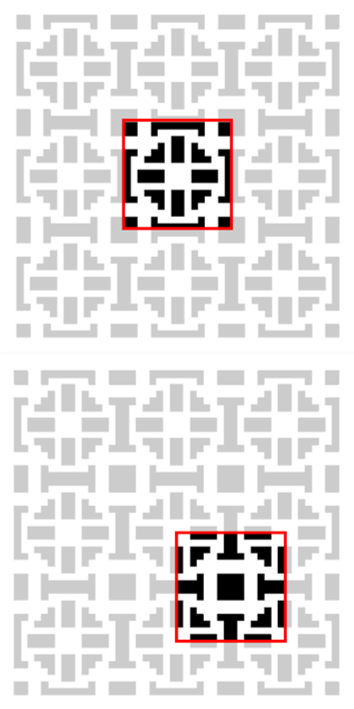
\includegraphics[width=1.0\linewidth]{images/TranslatedMicrostructureVertical.png}}
\end{wrapfigure}
After running the topology optimization algorithm, we generate a printable result by replacing each cell in the object lattice by a microstructure whose material properties match the optimal ones.

Material properties of the microstructures are computed using the homogenization theory which is more accurate with a smooth transition between the geometries of neighboring cells.
While smoothness in the material parameters can be easily enforced, it does not imply topological similarity of nearby microstructures. 
For example, any translation of a given microstructure in a periodic tiling will result in a microstructure geometrically different but with exactly the same mechanical properties. 
Fortunately, our database is very dense and multiple microstructures generally map to similar points in the material property space, offering several variants. To further increase the number of possibilities, we also incorporate an additional exemplar for each microstructure by translating it by half its size, which preserves its cubic or orthotropic symmetry without changing its properties (see inset Figure). We then run a simple but effective algorithm that picks the microstructure exemplars that minimize the boundary material mismatch across adjacent cells. We quantify this mismatch by $\mathcal{I}=\sum_{i=1}^{N_c} \mathcal{I}_i$, where $\mathcal{I}_i$ is the contribution associated to the cell $i$ and corresponds to the number of boundary voxels filled with materials that are different from the ones of the voxels' immediate neighbours across the interfaces.

Our algorithm proceeds as follows:
\begin{itemize}
\item For each cell, we define a list of possible candidates by picking all the microstructures mapping to material points lying in the vicinity of the optimal material point and we randomly initialize the cell with one of the candidates.
\item We compute the mismatch energy $\mathcal{I}_i$ associated to each cell $i$ and sort the cells according to their energy. 
\item We pick the first cell in the sorted list, i.e. the one with the highest energy and assign to it the microstructure candidate that decreases the energy the most. If we cannot decrease the cell energy, we move to the next cell in the list.
\item We update the mismatch energies of all the impacted cells and we update the priority list.
\item We repeat the last two steps until the mismatch energy $\mathcal{I}$ cannot be decreased anymore.
\end{itemize}

\section{Results and Discussion}
We first analyzed our microstructure sampling algorithm for 2D and 3D microstructure gamuts. Then we used these precomputed gamuts and we designed and optimized a wide variety of objects with our topology optimization algorithm.
\subsection{Microstructure Sampling}
We evaluated our method on two- and three-dimensional microstructures made of one or two materials. For the 2D case we considered patterns with cubic and orthotropic mechanical behaviors that can be described with 4 parameters (3 elasticity parameters and density) and 5 parameters (4 elasticity parameters and density) respectively. In 3D we computed the gamut corresponding to cubic structures with 4 parameters. In all cases, the size of the lattice for the microstructures was set to 16 in every dimension. We used isotropic base materials whose Young's modulus differed by a factor of 1000 and having 0.48 as Poisson's ratio. We initially computed the databases for two-material microstructures, but also adapted these databases for microstructures made of a void and a stiff material. In the later case, we replaced the softer material by void, filter out all the microstructures with disconnected components and, in the 3D case, filled the enclosed voids and recomputed the homogenized properties. We provide a comparison between the initial and postprocessed databases in the supplementary material. The resulting postprocessed gamuts are also depicted in Figure \ref{fig:gamuts}. 
Our databases contain 274k, 388k and 88k 2D cubic, 2D orthotropic and 3D cubic microstructures respectively and took from 15 hours to 93 hours to compute, which correspond to 68, 19 and 5 sampling cycles, respectively.
\begin{figure}
	\centering
	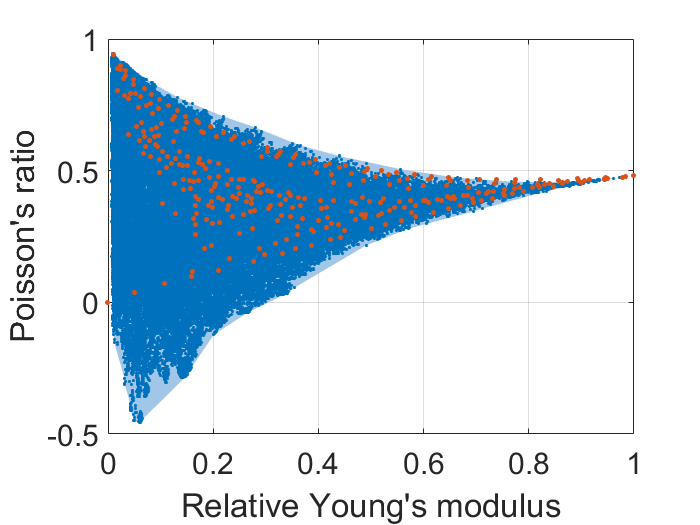
\includegraphics[width=.24\linewidth]{images/2D_cubic.png}
	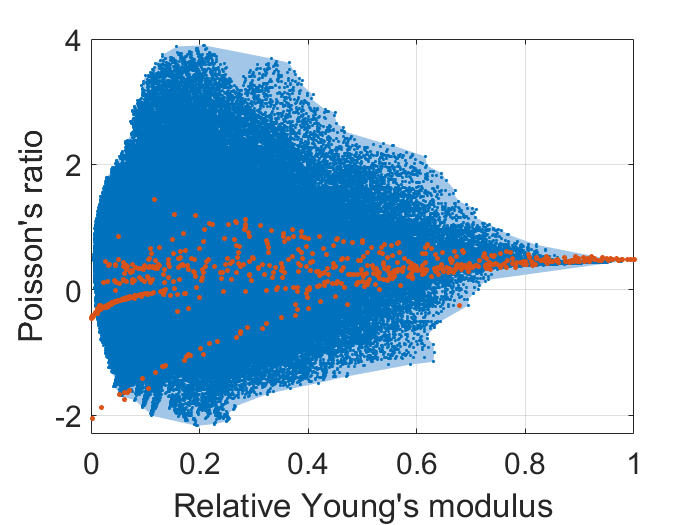
\includegraphics[width=.24\linewidth]{images/2D_ortho.png} 
	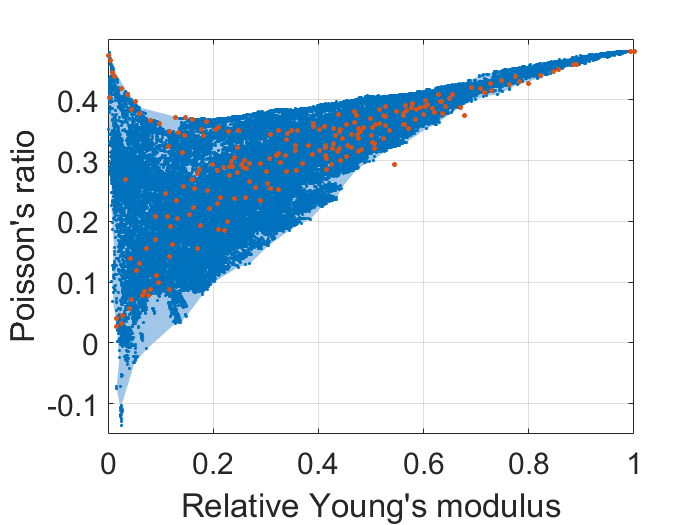
\includegraphics[width=.24\linewidth]{images/3D_cubic.png}
	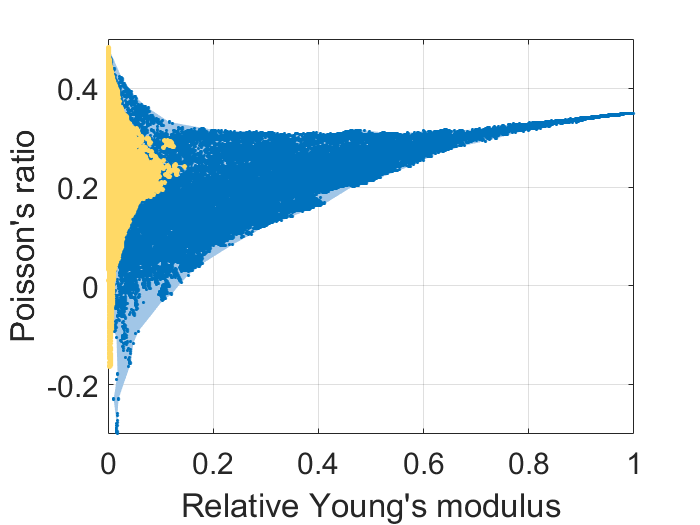
\includegraphics[width=.24\linewidth]{images/3D_cubic_Panetta.png}
	\caption{Gamuts computed with our discrete-continuous sampling scheme for 2D cubic structures (\emph{left}) , 2D orthotropic structures (\emph{second from left}), 3D cubic structures (\emph{second from right}) and 3D cubic structures with 0.35 as Poisson's ratio (\emph{right}). The plots show the results for the projection of the gamuts on the plane defined by the macroscale Young's modulus along the x axis (normalized by the Young's modulus of the stiffest base material) and the Poisson's ratio corresponding to a contraction along the y-direction when the material is stretched along the x-direction.
		The blue dots correspond to the generated samples,the orange dots correspond to the microstructures from~\citet{Schumacher:2015} and the yellow dots correspond to the microstructures from~\citet{Panetta:2015}.}
	\label{fig:gamuts}
\end{figure}
We first compared our results to the ones obtained by~\citet{Schumacher:2015}
and observed a significant increase in the coverage of the material space, even for 2D microstructures where we used a coarser discretization. This comforts us with the idea that topology optimization only, while helpful to locally improve the microstructure geometries, is suboptimal when one aims to discover the entire gamut of physical properties. The diversity of the microstructures that we obtained is also much richer, thus providing a larger set of options for the practical use of microstructures. Note that they employed some regularization to avoid thin features. For $16^3$ microstructures, we found regularization unnecessary since they are manifold and have a minimal feature size  of 1/16 of the lattice size, which is the same order of magnitude as the thinnest parts of Schumacher's microstructures.
For completeness, we also compared our database of 3D microstructures to the one of~\citet{Panetta:2015} at $16^3$ and $64^3$ grid resolutions (Figure \ref{fig:gamuts}, \emph{right}). Our initial database was computed with 0.48 as Poisson's ratio and is shown in the supplementary material. For this comparison, we then recomputed the material properties of the microstructures using the same Poisson's ratio as Panetta's, i.e 0.35, which affects the extremal values of the obtained gamut.
For the $64^3$ microstructures, we used morphological operations in the discrete step and sensitivity filtering with a radius of 3 voxels in the continuous step to limit the minimum feature size to 1/32 of the lattice size~\citep{sigmund:2007}. Note that this comparison is provided for reference only since our microstructures are cubic while Panetta's are isotropic (a subset of cubic). Furthermore, they target a different 3D printing technology with self-supporting constraints not imposed here.
Finally, we also obtained a dense sampling in the interior of the space, as a result of the randomness inherent to our approach. This reduces the need of running costly optimization in these areas and occurs even if we do not explicitly enforce any sampling there.

We also experimented with three-material 2D cubic microstructures (two solid materials with Young's moduli differing by a factor of 1000 and with 0.48 as Poisson's ratio, plus a void material). The resulting database contains about 800k microstructures that can potentially be printed. The corresponding gamut and some examples of the generated microstructures are shown in Figure \ref{fig:Cubic2D_3Materials}.
\begin{figure}
	\centering
	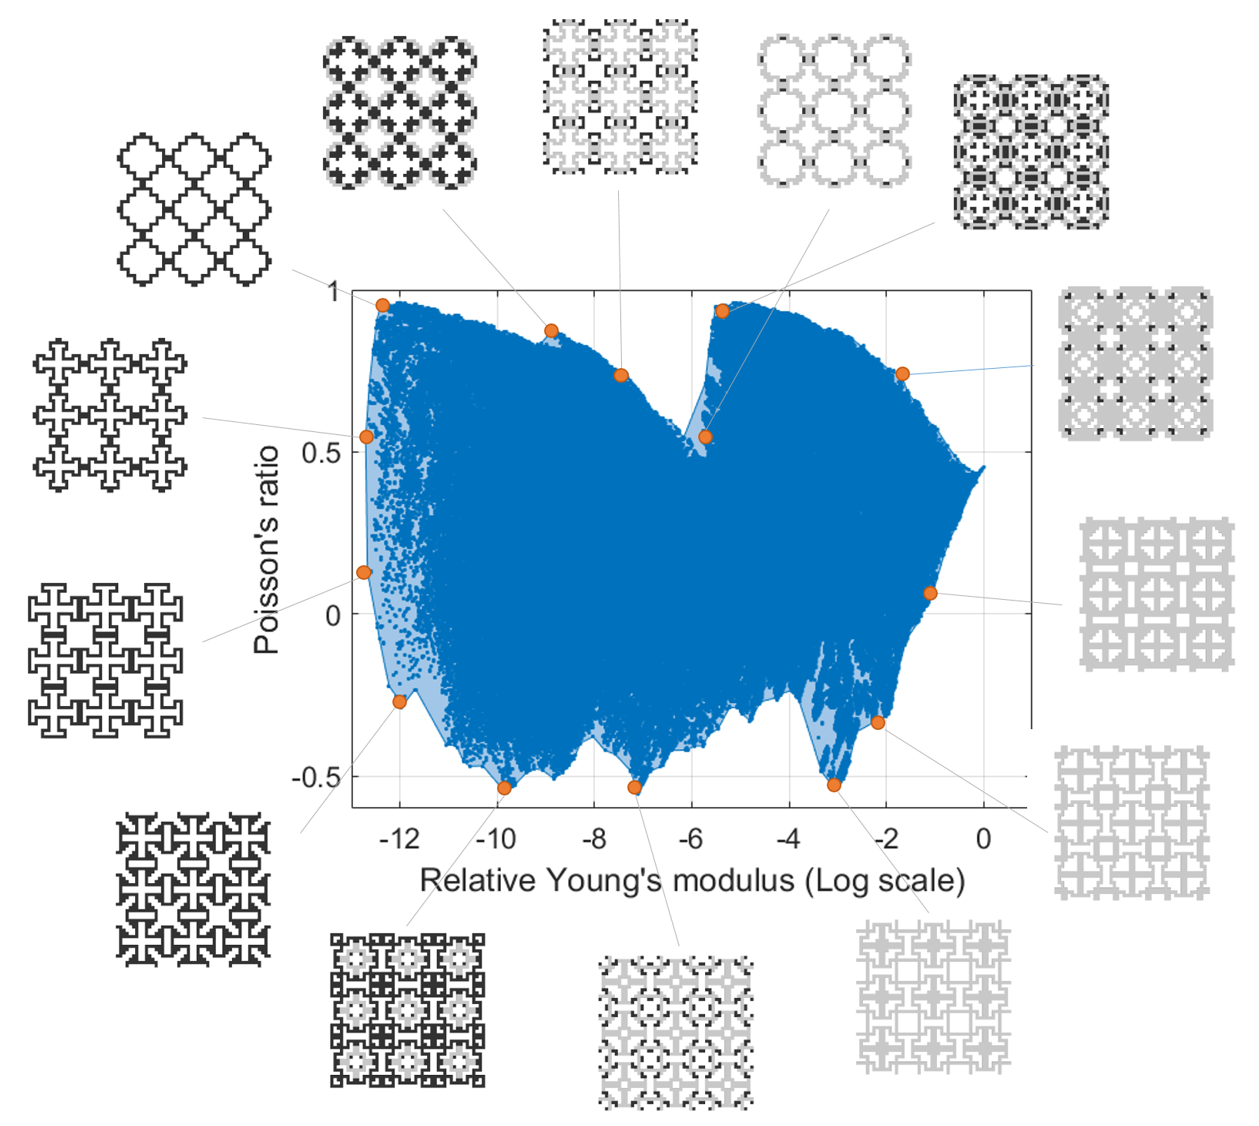
\includegraphics[width=.5\linewidth]{images/Cubic2D_3Materials.png}
	\caption{Gamut corresponding to 2D cubic microstructures made of two materials and void. The Young's modulus of the microstructures is plotted using a logarithmic scale. We show above some examples of microstructures lying near the estimated boundary of the gamut, i.e. with extreme material properties. The dark color corresponds to the softer material, while the light grey color is used for the stiffer material.}
	\label{fig:Cubic2D_3Materials}
\end{figure}
\subsection{Topology Optimization}
We tested our topology optimization algorithm on a number of simple test cases and large scale examples. Detailed analysis and discussion of the results is provided below.

\paragraph{Impact of the Material Space}
We evaluated the impact of the chosen material space on a 2D cantilever beam with optimized minimum compliance. We tested our topology optimization algorithm on isotropic, cubic and orthotropic gamuts as well as with the virtual materials used in the traditional SIMP approach and for which the stiffness of the material $E=\rho^p E_0$, $p \geq 1$ is a function of the density $\rho$ of the cell and the stiffness of the base material $E_0$. We also tested our algorithm on an analytical gamut with allowed stiffnesses $E$ defined by $E\leq \rho^3 E_0$. The results are shown in Figure \ref{fig:defo_cvg}. It can be noted that, as the dimension of the material space increases, the final energy of the system decreases. This is to be expected since higher dimensional space means larger gamuts.
Thus, when using cubic materials, the minimum compliance objective function reaches 3\% lower energy than the standard SIMP method with power index 3.
This difference reaches 11\% when we use orthotropic materials.
It is worth noting that the lowest elastic energy is achieved when we use the traditional SIMP method with $p=1$ (as shown in Figure \ref{plot:cvg}). However, this solution does not correspond to a realizable structure since some of the optimized materials do not correspond to any microstructure.
\begin{figure}
	\centering
	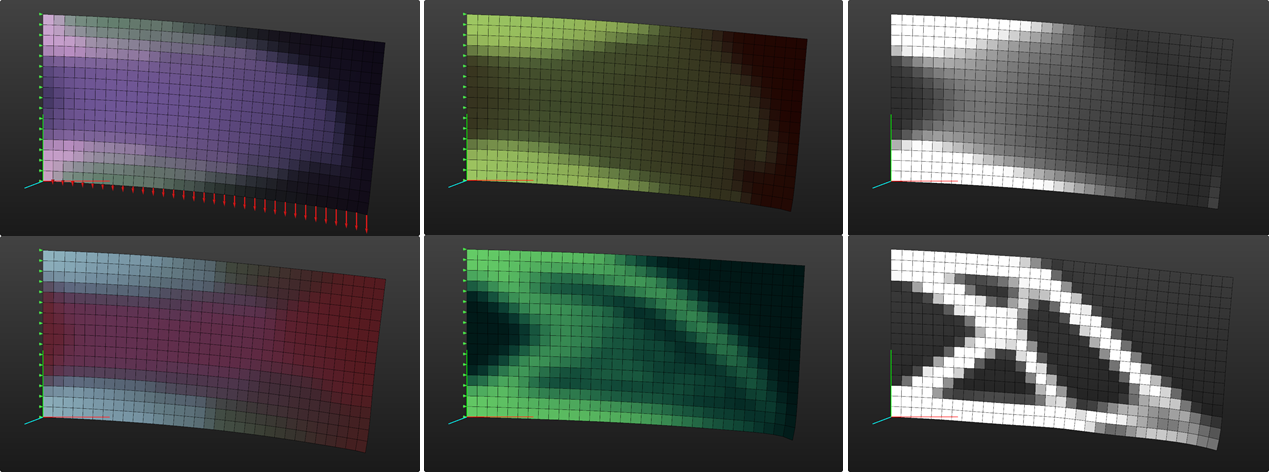
\includegraphics[width=0.95\textwidth]{images/cantilever.png}
	\caption{Material property distributions optimized in the orthotropic (\emph{top left}), cubic (\emph{bottom left}), isotropic (\emph{top middle}) and an analytically defined gamut $E \geq \rho^3 E_0$ (\emph{bottom middle}), with the material property space dimensions ranging from five to two. 
		We compare our algorithm with the standard SIMP method with power index $p=1$ (\emph{top right}) and $p=3$ (\emph{bottom right}). For these figures, we computed the color of each cell by mapping every base vector of the normalized parameter space to a color range and linearly interpolating the colors associated to each of the parameters.
		In this example, the left side of the cantilever is fixed while a force distribution is applied to the bottom side (see red arrows in the top left picture).}
	\label{fig:defo_cvg}
\end{figure}

\begin{figure}[h]
	\centering
	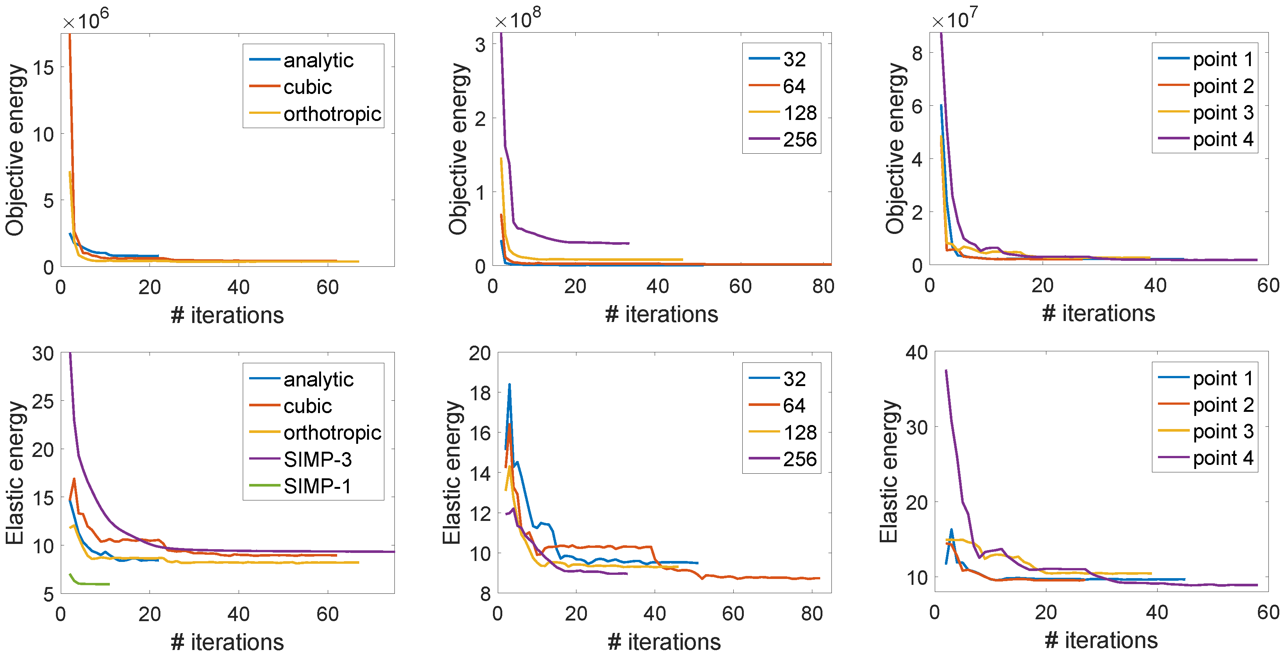
\includegraphics[width=0.95\textwidth]{figs/cvg_test.png}
	\caption{Convergence tests. Variation of the objective energy (\emph{left}) and the elastic energy \emph{right} of a beam being optimized for minimum compliance as the optimization progresses. The convergence plots correspond to the beam of Figure \ref{fig:defo_cvg} when optimized using different material spaces (\emph{top}), different resolutions for the beam lattice (\emph{middle}) when using cubic microstructures, and different initial material properties for the cubic microstructures (\emph{bottom}).}
	\label{plot:cvg}
\end{figure}
\begin{figure}
	\centering
	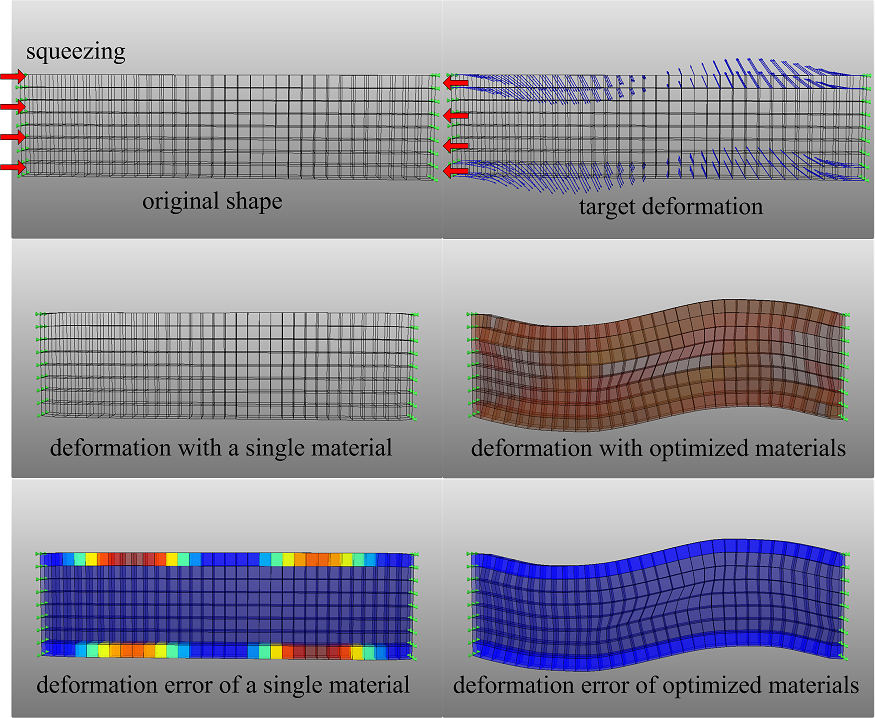
\includegraphics[width=.5\linewidth]{images/bar_visio_new.png}
	\caption{
		Optimizing a beam to take an ``S'' shape under compression.
		A beam with homogeneous material can only compress uniformly (left column).
		The optimized beam can deform as requested (right column).
		Target displacements are set on the horizontal boundary cells.
		The color plot for the bottom beams shows the deformation error of each cell defined by Equation~\ref{eq:td}.
		\label{fig:beam_S_shape}}
\end{figure}

\paragraph{Matching Quality}
	We evaluated for different examples the matching quality of the target deformation optimization.
	For the first test, we forced a beam to take an `S' shape when undergoing tensile forces (Figure \ref{fig:beam_S_shape}). In order to avoid overfitting, we applied target displacements on the vertices of the boundary cells only. As depicted in the figure, the use of microstructures largely improves the global shape of the beam, which closely matches the target deformed shape. This becomes even more striking when compared to the behavior of a beam made of a homogeneous material.
		We also validated our algorithm by designing a soft ray whose wings can flap using a compliant mechanism (see Figure \ref{fig:ray} and accompanying video). Boundary conditions are applied on two circular areas located along the spine of the ray. Each disk has one degree of freedom for deformation, namely contracting or expanding along the disk normals. This mechanism resembles the one of many hydraulics-driven soft robots. We define two target deformation objectives corresponding to the flapping of the wings up and down, when alternatively contracting and expanding the two disks' boundaries. By running our multi-objective topology optimization framework, we can compute an optimized material design that can achieve both deformation modes when the corresponding boundary conditions are exerted.

\begin{figure}[t]
	\centering
	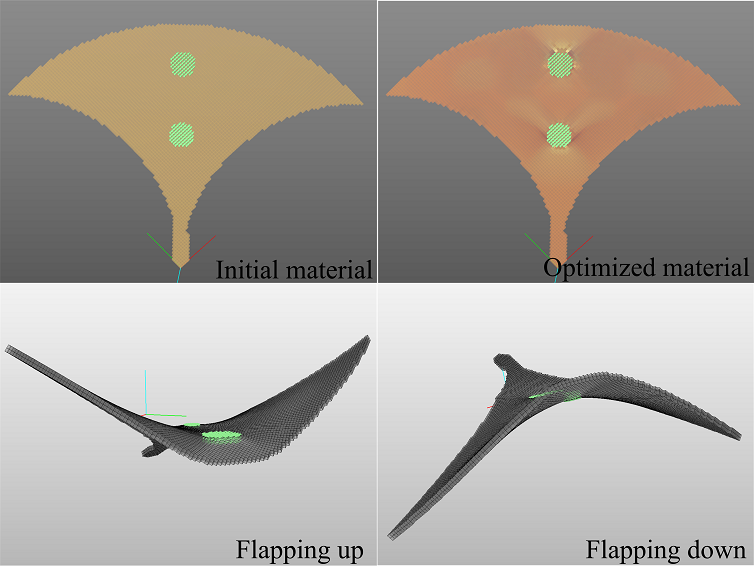
\includegraphics[width=.6\linewidth]{images/ray.png}
	\caption{Designing a soft ray. The wings of the ray flap up and down when cells on its spine contract and expand.
	Constrained vertices are colored in green.
	The deformations achieved with the optimized materials are displayed on the bottom row.}
	\label{fig:ray}
\end{figure}
\paragraph{Convergence and Robustness}
We evaluated the convergence rate of our topology optimization both on the minimum compliance problem and with the target deformation objective. For the minimum compliance problem, we used the same loading as the one of Figure \ref{fig:defo_cvg}. The corresponding results are shown in Figure~\ref{plot:cvg} where we plot both the deformation energy of the structure as defined in Equation \ref{eq:mc} and the original objective of the problem \ref{eq:op} that also includes the volume term defined by Equation \ref{eq:vol}. For all these examples, the algorithm converged after a couple of dozen iterations, irrespectively of the lattice resolution, i.e. the number of variables and the number of non-linear constraints. This demonstrates the scalability of the our algorithm. We also tested the robustness of our algorithm by starting with different initial conditions. In this case, we initialized the material parameters of each cell with a random material point projected onto the boundary of the gamut. Similar to other topology optimization schemes, we have no guarantee that we reach the global minimum of the function, and indeed, our algorithm sometimes converges to different solutions. However we note that these different solutions have a similar final objective value and are therefore equally good.

For the evaluation of the target deformation optimization, we tested the convergence rate when optimizing for functional mechanisms.
To this end, we designed several grippers that can grasp objects by moving their tips when external forces are applied to their extremities. We experimented with four sets of boundary conditions, namely, pulling and pushing the back of the gripper horizontally, and compressing and stretching the extremities of the gripper vertically. As shown in Figure \ref{fig:gripper}, these different settings lead to different material structures. The deformation errors of all the four designs converge to a low level after a couple of hundreds of iterations.

\begin{figure}[t]
	\centering
	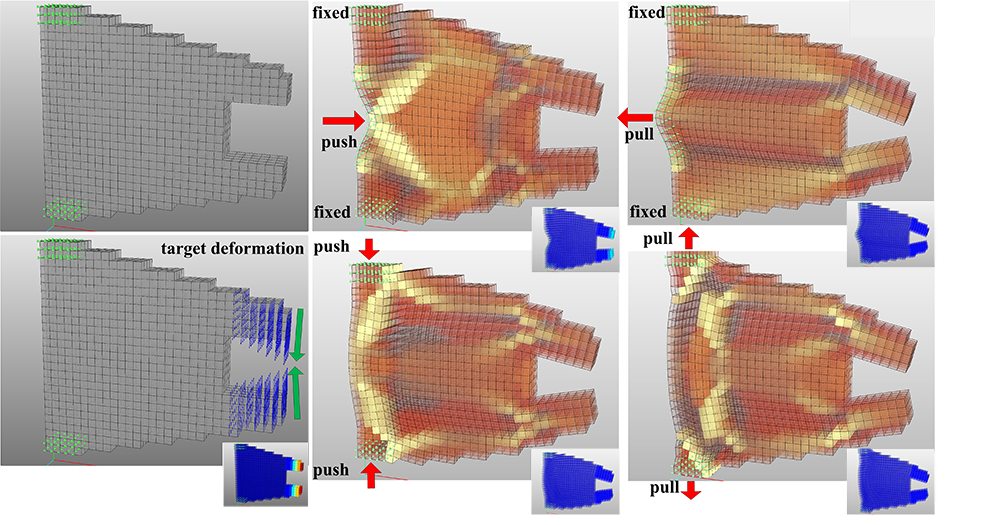
\includegraphics[width=.9\linewidth]{images/gripperVar.png}
	\caption{Designing functional grippers. The left column shows the rest shape of the gripper and the target deformation for the tip.
	The green dots correspond to the fixed vertices while the blue arrows are the target displacements.
	The middle and right columns correspond to the optimized results obtained for the specified boundary conditions.
	The inset pictures color-code the initial and final deformation error for the different examples.
	The convergence plots in the bottom row depict the change in the sum of the deformation errors corresponding to all the cells (left) and the value of the maximal cell error contribution (right) as the optimization progresses.}  
	\label{fig:gripper}
\end{figure}
\paragraph{Accuracy}
\begin{figure}
	\centering
	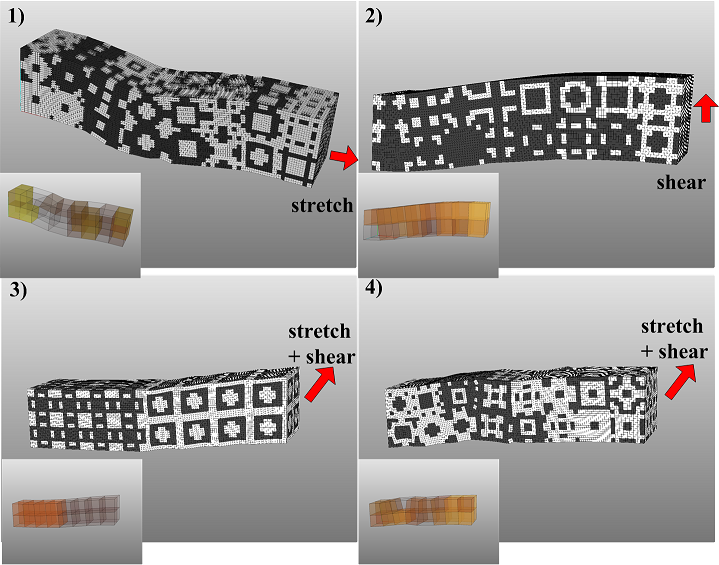
\includegraphics[width=.6\linewidth]{images/hom_beam.png}	
	\caption{Comparison of simulated beams with homogenized material properties (\emph{inset pictures}) to the ones using full microstructures (\emph{large pictures}).
		}\label{fig:hom_beam}
\end{figure}

\begin{figure}[h]
	\centering
	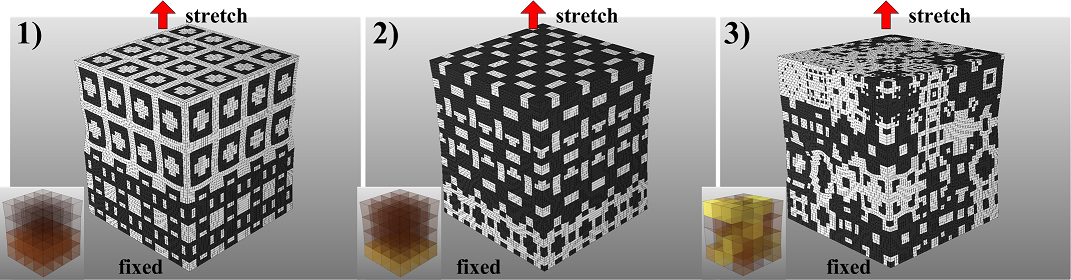
\includegraphics[width=.6\linewidth]{images/hom_cube_random.png}	
	\caption{Comparison of simulated cubes with different material patterns modeled by homogenized cells (\emph{inset pictures}) and full resolution microstructures (\emph{large pictures}).}
		\label{fig:hom_cube_2}
\end{figure}

We evaluated the accuracy of our algorithm on several optimized structures by comparing the deformation obtained when using the optimized homogenized material properties for each cell to the one obtained by a high resolution simulation in which every cell is replaced by its mapped microstructure.
We first evaluated the accuracy on a deformable bar, one side of which was rigidly attached while the other was subject to different sets of external conditions (see Figure \ref{fig:hom_beam}). We used a $8\times2\times2$ lattice to represent the bar with homogenized cells, which translates into a $128\times32\times32$ grid for the full resolution mesh. Similar stretching, bending and shearing behaviors were obtained for both sets of models. From a quantitative point of view, the differences amount to 5-10\% in terms of average vertex displacement and 9\%-33\% in terms of elastic deformation energy (see Table \ref{tab:hom}). We further evaluated the effects of material patterns by running a similar comparison on a cube made of periodic layers of similar microstructures and with random assignments of microstructures (Figure \ref{fig:hom_cube_2}).  As reported in Table \ref{tab:hom}, we show that the ratio between the magnitudes of the average vertex displacement differences is between 4\% and 7\%, and the elastic energy difference is between 10\% and 19\%.

Finally, we also compared the behaviors of one of the grippers (Figure \ref{fig:gripper_validate}). The original optimized gripper is made of 3k elements while the high resolution version is made of 4M voxels.
Overall, the two models exhibit similar global deformation behaviors, in particular in the tip area. Some differences can be observed on the left side of the gripper for which the high-resolution model exhibits a lower effective material stiffness than its homogenized counterpart. With the same displacement boundary conditions applied, the high-resolution model deforms about 25\% more than the homogenized model.
	
	\begin{figure}[t]
		\centering
		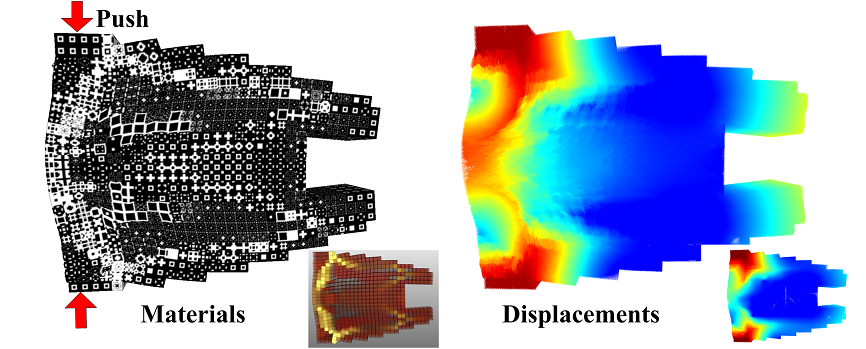
\includegraphics[width=.99\linewidth]{figures/gripper_cmp.png}	
		\caption{\updated{Comparison of a simulated gripper with homogenized material properties (\emph{inset picture, left}) to the one using full microstructures (\emph{main picture, left}). The figures on the right show the vector field of vertex displacement of the two models. The blue-to-red colors represent the magnitudes of the displacements.}
			\label{fig:gripper_validate}}
	\end{figure}
	
	\begin{figure}[h]
		\centering
		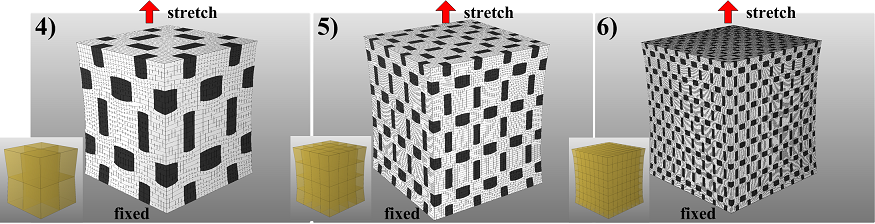
\includegraphics[width=.99\linewidth]{figures/hom_cube_peri.png}	
		\caption{\updated{Simulation of a cube made of a periodic arrangement of a single microstructure at different resolutions. Inset pictures correspond to the model with homogenized material properties, while main pictures correspond to the full resolution simulations.}
			\label{fig:hom_cube_1}}
	\end{figure}
	
The differences observed between the homogenized model behaviour and the full resolution simulation can be explained by two major factors: (i) numeral stiffness when using larger elements which tends to make the homogenized mesh slightly stiffer in particular when bending deformation arises, (ii) violation of the periodicity assumption when replacing each cell by a single microstructure. This issue can be reduced by replacing each cell by a {\it tiling} of microstructures. This was verified on a cube made of a periodic arrangement of a single microstructure (see Figure \ref{fig:hom_cube_1}). And indeed, as we increase the resolution of the simulation grid, the error between the homogenized model and the full resolution version decreases and converges to similar values. }

\paragraph{Orthotropic materials}
We tested the behavior of our algorithm in a 5-dimensional space by using the gamut of 2D orthotropic microstructures depicted in Figure \ref{fig:gamuts} (\emph{middle}). To this end, we used a regular lattice whose vertices on the left side where fixed and we applied parallel forces on the vertices of the opposite side. The goal in the test was to minimize the compliance of the structure. As can be seen in Figure \ref{plot:res} and in the accompanying video, we experimented with different force directions. Unsurprisingly, when a single cell is considered, the microstructure that we obtain has a structure that is aligned with the direction of the forces (see Figure \ref{plot:res}, \emph{left}). 
For a higher resolution lattice this is no longer true and the resulting overall structure becomes less intuitive (see Figure \ref{plot:res}, \emph{right}). 
Note that the resulting material distribution varies smoothly. By considering various alternative for each material point, our tiling algorithm is able to map the material properties to microstructures which are well connected. 

\begin{figure}
	\centering
	\sixfigure{.16\textwidth}{.03in}{figures/ortho_cell0.png}{figures/ortho_cell1.png}{figures/ortho_cube_ms0.png}{figures/ortho_cube_ms6.png}{figures/ortho_cube_ms40.png}{figures/ortho_cube_ms51.png}
	\sixfigure{.16\textwidth}{.03in}{figures/ortho_cell2.png}{figures/ortho_cell3.png}{figures/ortho_cube_mat0.png}{figures/ortho_cube_mat6.png}{figures/ortho_cube_mat40.png}{figures/ortho_cube_mat51.png}
	\caption{Optimizing the orthotropic material parameters of a single cell (\emph{left}) and a $32\times32$ lattice of cells (\emph{right}) subject to directional forces. The vertices on the left side of the layout are fixed while forces are applied on the right vertices as depicted by the red arrows. Our simple but effective tiling algorithm allows to nicely transition between microstructures of smoothly material properties (\emph{right, top}).}
	\label{plot:res}
\end{figure}

\begin{table}
	\centering
	\footnotesize
	\caption{\updated{Error statistics (SI units). The size of one microstructure is set to $1\times1\times1$.}} 
	{\begin{tabularx}{\linewidth}{ |X| X | X | X | X | }
			\hline
			Example & Mean displacement & Mean displacement difference & \multicolumn{2}{p{3.2cm}|}{\centering Elastic energy \newline homogenized/full resolution}\\ \hline
			Beam 1 & 6.47$\times10^{-3}$ & 6.04$\times10^{-4}$ & 6.85$\times10^{-5}$ & 6.17$\times10^{-5}$ \\
			Beam 2 & 6.47$\times10^{-3}$ & 6.04$\times10^{-4}$ & 1.63$\times10^{-5}$ & 1.08$\times10^{-5}$ \\
			Beam 3 & 5.07$\times10^{-3}$ & 4.97$\times10^{-4}$ & 2.38$\times10^{-4}$ & 2.07$\times10^{-4}$ \\
			Beam 4 & 8.78$\times10^{-3}$ & 4.45$\times10^{-4}$ & 3.33$\times10^{-4}$ & 2.30$\times10^{-4}$ \\
			Cube 1 & 3.62$\times10^{-3}$ & 2.86$\times10^{-4}$ & 3.64$\times10^{-3}$ & 3.20$\times10^{-3}$ \\
			Cube 2 & 4.35$\times10^{-3}$ & 1.94$\times10^{-4}$ & 6.82$\times10^{-3}$ & 5.94$\times10^{-3}$ \\
			Cube 3 & 5.42$\times10^{-3}$ & 4.22$\times10^{-4}$ & 7.81$\times10^{-3}$ & 6.32$\times10^{-3}$ \\
			Gripper& 1.32$\times10^{-2}$ & 6.90$\times10^{-3}$ & 8.67$\times10^{-3}$ & 5.70$\times10^{-3}$ \\
			Cube 4 & 5.22$\times10^{-3}$ & 4.89$\times10^{-4}$ & 2.08$\times10^{-2}$ & 1.63$\times10^{-2}$ \\
			Cube 5 & 5.21$\times10^{-3}$ & 2.17$\times10^{-4}$ & 1.89$\times10^{-2}$ & 1.63$\times10^{-2}$ \\
			Cube 6 & 5.21$\times10^{-3}$ & 1.32$\times10^{-4}$ & 1.82$\times10^{-2}$ & 1.63$\times10^{-2}$ \\
			\hline
		\end{tabularx} }
		\label{tab:hom}
	\end{table}
	
	\subsection{3D-Printed Designs}
	
	Leveraging our two-scale approach, we used our topology optimization algorithm to generate a wide variety of high resolution models that we 3D-printed. We used a Stratasys Objet Connex 500 and the two base materials \emph{Vero Clear} and \emph{Tango Black Plus} and used the database containing the three-dimensional cubic microstructures. The sizes and computation times of the resulting models are outlined in Table \ref{tab:results}. 
	
	Since Ipopt performs a line search at each gradient step, one single step may correspond to multiple simulations. We show the average time required for taking a step in the last column of Table \ref{tab:results}. For these large scale examples, Ipopt takes two hundred iterations in average to find a local minimum. 
	Since our problem is formulated as a very general constrained continuous optimization, it is independent of the optimization package that is used and its speed could potentially be further improved by using alternative minimizers. 
	We found Ipopt to be a good choice for its capability to efficiently handle a large number of inequality constraints, which is not the case of other popular minimizers used in topology optimization such as the method of moving asymptotes (MMA).
	
	Our algorithm is mainly directed towards engineering applications and targets the design of objects undergoing small deformations. In the following examples, we sometimes intentionally exaggerated the target displacements (and scaled the external forces accordingly) for better visualization, which does not change the output of the algorithm with a linear material model.
	
	\begin{table}
		\centering
		\footnotesize
		\caption{Statistics on the 3D-printed models. The last row uses the database of $64^3$ microstructures.} 
		{
			\begin{tabularx}{\linewidth}{ |X| X | X | p{1cm}| p{1cm}| }
				\hline
				Example & Grid Size & \# Voxels & Time per FEM Solve [s] & Time per Step [s]\\ \hline
				Beam   & 96$\times$24$\times$4  & 38M  &  0.7 & 5\\
				Flexure & 32$\times$32$\times$16 & 67M  & 1 & 12\\
				Gripper   & 64$\times$32$\times$8  & 67M  & 1.7 & 10\\	\hline
				Bunny & 32$\times$32$\times$32 & 134M  & 0.6 & 4 \\
				Bridge & 128$\times$64$\times$32 & 1074M  & 27 & 81\\
				Bridge 2 & 320$\times$160$\times$80 & 1074G  & 1.3k & - \\
				\hline
			\end{tabularx} }
			\label{tab:results}
		\end{table}
		
		\paragraph*{Beams with controlled deformation behaviour}
		
		We started by designing a 3D hollowed beam with a desired deformed shape. The beam was stretched by moving vertices on two opposite sides. Our topology optimization algorithm was run using a target deformation objective. The resulting optimized material properties and the 3D-printed structure are depicted in Figure \ref{fig:beam}. 
		
		\begin{figure}[h!]
			\centering
			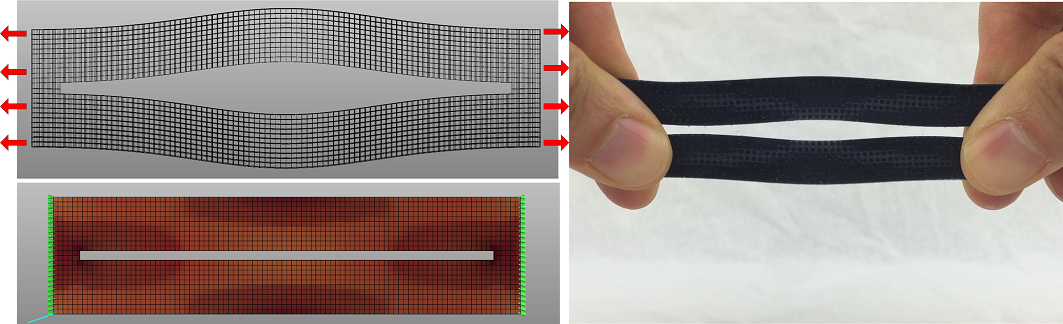
\includegraphics[width=.99\linewidth]{figures/bar2_two.png}
			\caption{
				An optimized hollow beam with target deformation. The left figure shows the target deformation and optimized material distribution. The right figure shows the 3D-printed structure and the achieved deformation.
				\label{fig:beam}}
		\end{figure}
		
		\paragraph*{Multi-Objective Flexure Design}
		We tested our algorithm on a multi-target deformation setting by optimizing the structure of a flexure mount with two different target shapes (see Figure \ref{fig:flexure}). Here, our goal is to design a flexure that resists vertical loads while remaining compliant to horizontal loads. We assume that the object mounted on the flexure is connected to the flexure using a cylindrical connector that transmits the forces to the flexure via the connecting area. In the first scenario, vertical forces are applied to the points of the cylindrical area and we ask the flexure to stay as close as possible to its rest configuration. In the second scenario, horizontal forces are applied to the points of the cylinder and we ask the flexure shape to match the shape shown in the Figure \ref{fig:flexure}. %\melina{how was this shape obtained?}.
		\begin{figure}
			\centering
			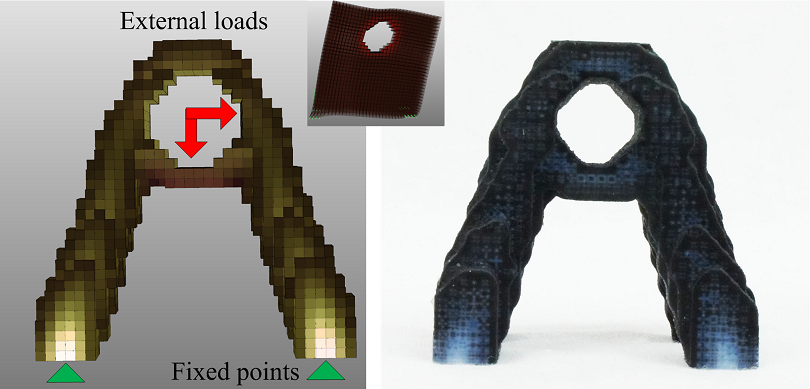
\includegraphics[width=.99\linewidth]{figures/flex_four.png}	
			\caption{Optimizing a flexure mount. The flexure is connected to an object thanks to a cylindrical connector. We leave space for this connector by keeping a cylindrical area of the design layout empty of material. The material distribution of the flexure is optimized for two sets of external forces applied to the cylindrical area. Under vertical load, the flexure should stay close to the rest shape while under horizontal load, the flexure should deform according to the inset figure. 
				\label{fig:flexure}}
		\end{figure}
		
		\begin{figure}[h]
			\centering
			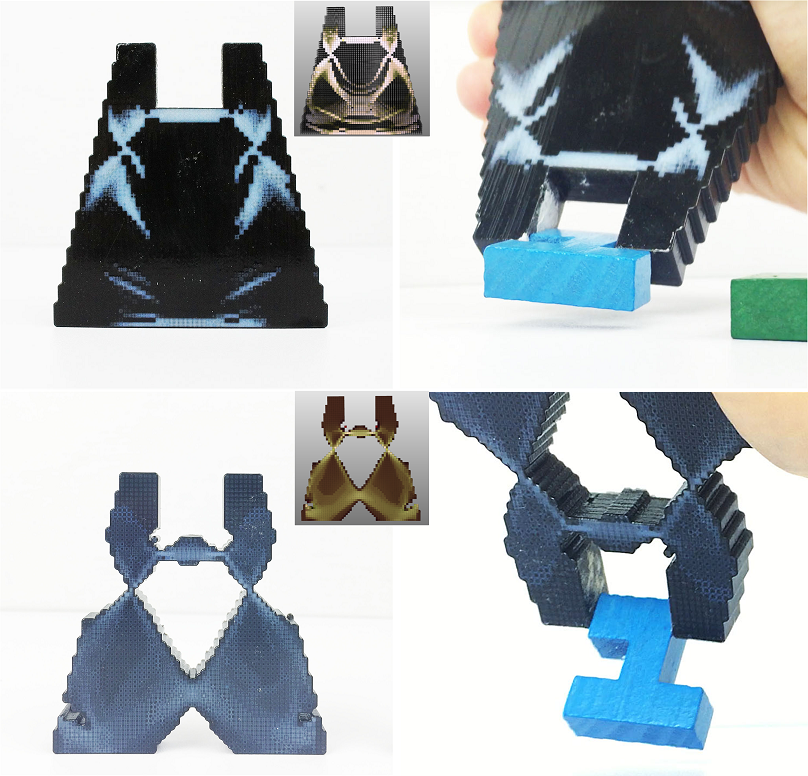
\includegraphics[width=.99\linewidth]{figures/gripper_print.png}
			\caption{3D-printed functional grippers. By setting different target ratios of the rigid material, different designs can be obtained. 
				When more soft material is used the grasping behaviour of the gripper is obtained via out-of-plane bending (\emph{top}), whereas more rigid material is used, the gripper deformation remains planar (\emph{bottom}).}  
			
			\label{fig:gripper_printed}
		\end{figure}
		
		\paragraph{Gripper}
		We verified the functionality of our grippers by fabricating two of them. For these results we ran the optimization on high resolution meshes of the version that grasps the object when the extremities of the gripper are pressed (see Figure \ref{fig:gripper_printed}). By changing the parameter controlling the ratio of the soft material, different designs based on different mechanisms can be achieved. When more soft material is used the gripper achieves its target deformation thanks to out-of-plane bending, while for stiffer designs, the grasping motion is achieved via in-plane deformation.
		\paragraph*{Minimal Compliance Examples}
		To demonstrate the scalability of our algorithm, we ran our topology optimization algorithm on a Stanford bunny (Figure \ref{fig:bunny}) made of more than 100 million voxels and subject to two load case scenarios.
		We also designed two bridges of increasing resolutions. The first bridge was optimized using a lattice of half a million cells which corresponds to 1 billion voxels (Figure \ref{fig:bridge}). For the second bridge, we used the database of $64^3$ microstructures and a layout made of 4 million cells, which amounts to 1 trillion voxels. We initialized the topology optimization by running the algorithm on a lower resolution grid with 1.4 million elements and used the resulting parameters as initial material parameter values for the higher resolution optimization. 	
		\begin{figure}
			\centering	
			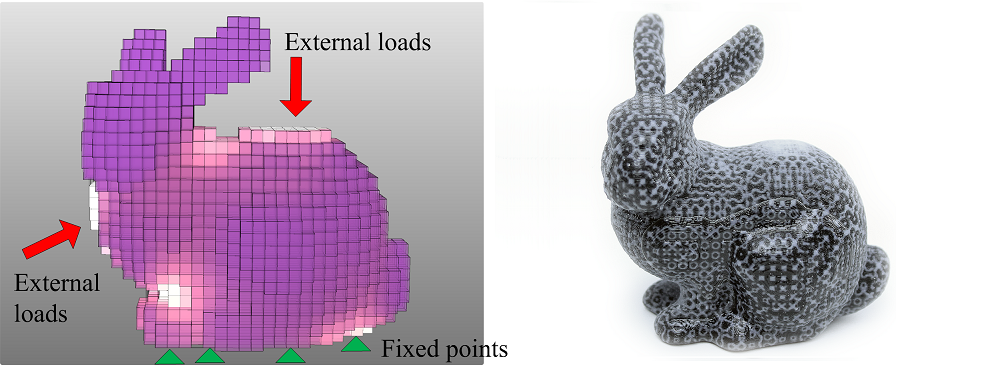
\includegraphics[width=.99\linewidth]{figures/bunny_two.png}
			\caption{Stanford bunny optimized for two loading cases. Two sets of external forces are applied to the back and chest of the bunny as indicated by the arrows, and the color indicates the material distribution (\emph{left}). Material parameters are mapped to microstructures to obtain an object that can be actually printed (right).
				\label{fig:bunny}}
		\end{figure}
		
		\begin{figure}
			\centering
			%\twofigure{.235\textwidth}{.03in}{figures/bridge_bdry.png}{figures/bridge2.jpg}
			%\twofigure{.235\textwidth}{.03in}{figures/bridge3.jpg}{figures/bridge2.jpg}	
			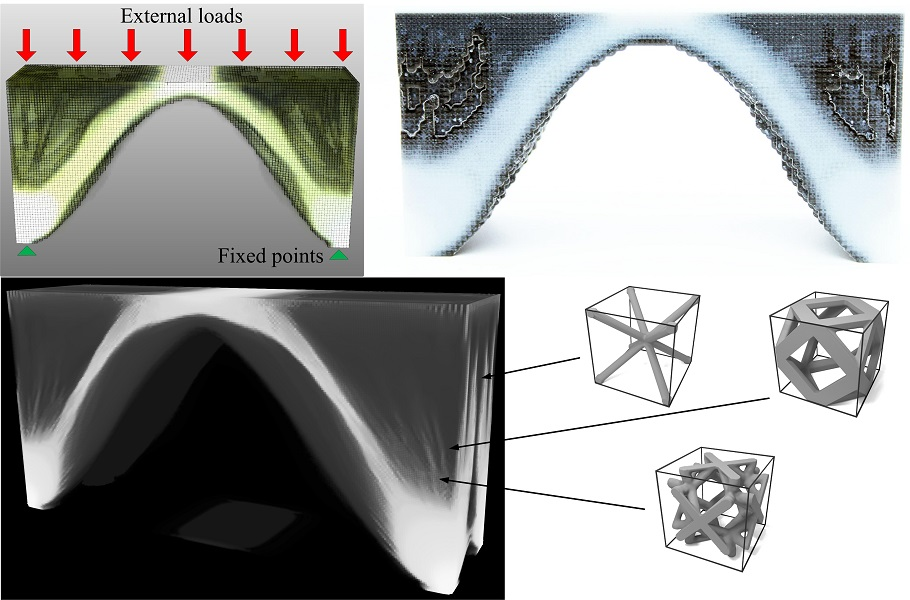
\includegraphics[width=.99\linewidth]{figures/bridge_three.jpg}
			\caption{Optimizing a bridge. The initial layout corresponds to a 128x64x32 regular grid. We apply uniform loads on the upper plane deck. We compute the material parameters and set cells with extremely low stiffness to void (\emph{top left}). We look up the microstructures and 3D print the bridge (\emph{top right}). We scaled the problem to 1 trillion voxels by using a lattice of 4 million elements where each element corresponds to a $64^3$ microstructure (bottom).
				\label{fig:bridge}}
		\end{figure}